\chapter{Von den Quanten offener Strings zu Tachyonen und Gravitation}

\lectureoverview{Wir quantisieren nun die Normalschwingungen aus der vorigen Vorlesung und fragen, welche Teilchenzustände sie hervorbringen. Jede transversale Mode ist ein harmonischer Oszillator, doch ihre Normierung ist etwas ungewohnt: Wird die Mode \(n\) angeregt, steigt die Energie im Lichtkegelkoordinatensystem und damit auch das Massenniveau zum Quadrat um \(n\) Einheiten. Das erste angeregte Niveau des offenen Strings transformiert genau wie die beiden transversalen Polarisationen eines masselosen Vektors. Die relativistische Konsistenz legt daher fest, dass das Quadrat der Masse des Grundzustands negativ ist. Dieser Zustand ist das Tachyon des bosonischen Strings; seine eigentliche Bedeutung ist ein instabiles Vakuum, nicht ein praktisch nutzbares überlichtschnelles Teilchen. Sobald Strings miteinander wechselwirken, sind geschlossene Strings durch das Zusammenfügen und Aufspalten unvermeidlich; die niedrigste Anregung eines geschlossenen Strings wird das Graviton sein.}

\section{Der in jeder Stringmode verborgene Oszillator}

Für eine transversale Koordinate \(X\) hat die \(n\)te nichtverschwindende Normalschwingung die Energie und die Lagrange-Funktion

\begin{align}
  E_n
  &=
  \frac14\dot X_n^{\,2}
  +\frac{n^2}{4}X_n^2,
  \label{eq:l03-mode-energy}\\
  L_n
  &=
  \frac14\dot X_n^{\,2}
  -\frac{n^2}{4}X_n^2.
  \label{eq:l03-mode-lagrangian}
\end{align}

Die Faktoren \(1/4\) sind kein Fehler. Sie spiegeln die Normierung wider, die sich ergibt, wenn man die Stringwirkung in unabhängige Fourier-Moden zerlegt. Der erste Schritt zur Konstruktion des Hamiltonoperators besteht daher darin, den kanonischen Impuls zu berechnen:

\begin{equation}
  p_n=\frac{\partial L_n}{\partial\dot X_n}
     =\frac12\dot X_n,
  \qquad
  \dot X_n=2p_n.
  \label{eq:l03-canonical-momentum}
\end{equation}

Die Legendre-Transformation ergibt

\begin{equation}
  H_n=p_n\dot X_n-L_n
     =p_n^2+\frac{n^2}{4}X_n^2.
  \label{eq:l03-mode-hamiltonian}
\end{equation}

\begin{figure}[H]
  \centering
  \includegraphics[width=0.82\textwidth]{lecture_03_figure_01.png}
  \caption{Energie, Lagrange-Funktion, kanonischer Impuls und Hamiltonoperator der Mode in der vom offenen String übernommenen Normierung.}
  \lectureframe{00:05:40}
  \label{fig:l03-mode-hamiltonian-board}
\end{figure}

Um \(H_n\) zu faktorisieren, kombinieren wir \(X_n\) und \(p_n\) wie folgt:

\begin{equation}
  \frac{nX_n}{2}\pm i p_n.
\end{equation}

Klassisch würden die beiden Faktoren kommutieren, quantenmechanisch gilt jedoch

\begin{equation}
  [X_n,p_m]=i\delta_{nm}
  \label{eq:l03-canonical-commutator}
\end{equation}

in Einheiten mit \(\hbar=1\). Die gemischten Terme heben sich nicht einfach auf. Für eine feste Mode gilt:

\begin{align}
  \left[\frac{nX_n}{2}+ip_n,
        \frac{nX_n}{2}-ip_n\right]
  &=n,
  \label{eq:l03-unscaled-commutator}\\
  \left(\frac{nX_n}{2}-ip_n\right)
  \left(\frac{nX_n}{2}+ip_n\right)
  &=H_n-\frac n2.
  \label{eq:l03-factorized-hamiltonian}
\end{align}

\begin{figure}[H]
  \centering
  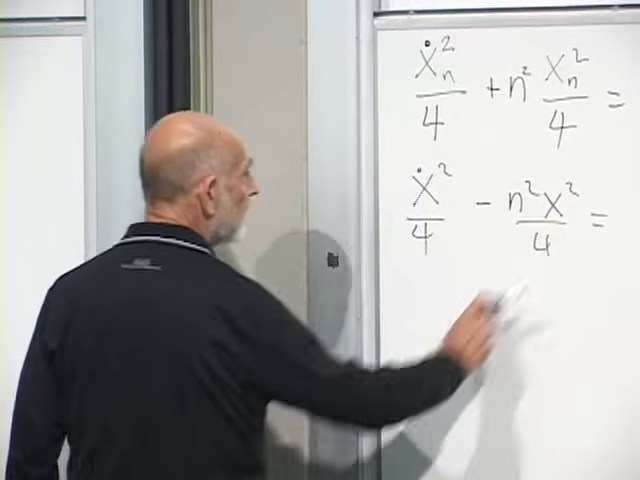
\includegraphics[width=0.82\textwidth]{lecture_03_figure_02.png}
  \caption{Die Rechnung an der Tafel, bei der der kanonische Kommutator den Faktor \(n\) liefert.}
  \lectureframe{00:10:30}
  \label{fig:l03-commutator-board}
\end{figure}

Der Faktor \(n\) gibt vor, wie die Leiteroperatoren zu normieren sind:

\begin{align}
  a_n
  &\equiv
  \frac{\sqrt n}{2}X_n+\frac{i}{\sqrt n}p_n,
  \label{eq:l03-annihilator}\\
  a_n^\dagger
  &\equiv
  \frac{\sqrt n}{2}X_n-\frac{i}{\sqrt n}p_n.
  \label{eq:l03-creator}
\end{align}

Sie erfüllen

\begin{equation}
  [a_n,a_m^\dagger]=\delta_{nm},
  \qquad
  H_n=n\left(a_n^\dagger a_n+\frac12\right).
  \label{eq:l03-oscillator-algebra}
\end{equation}

Somit fügt \(a_n^\dagger\) dem \(n\)ten Oszillator ein Quant hinzu, das jedoch \(n\) Einheiten der Modenenergie trägt. Der vertraute Abstand der Oszillatorniveaus bleibt erhalten; seine Frequenz ist \(\omega_n=n\).

\begin{figure}[H]
  \centering
  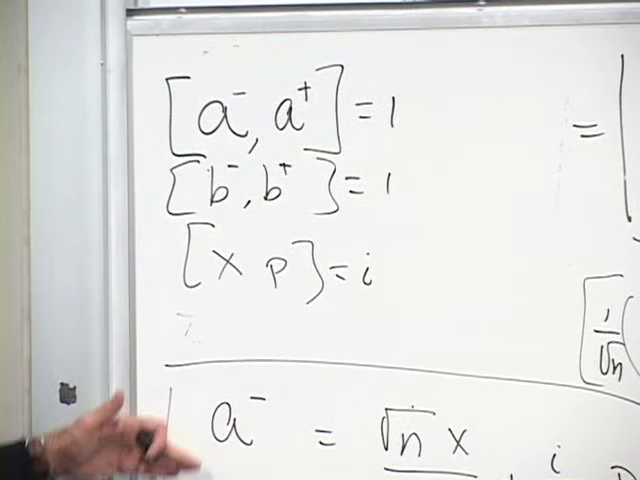
\includegraphics[width=0.82\textwidth]{lecture_03_figure_03.png}
  \caption{Normierte Vernichtungs- und Erzeugungsoperatoren des \(n\)ten Stringoszillators.}
  \lectureframe{00:12:00}
  \label{fig:l03-ladder-board}
\end{figure}

\subsection{Zwei transversale Türme}

In vier Raumzeitdimensionen hat ein String, der sich mit sehr großem Impuls entlang der \(z\)-Achse bewegt, zwei transversale Koordinaten, \(X\) und \(Y\). Wir benötigen daher zwei unabhängige Oszillatortürme. Die Operatoren \(a_n,a_n^\dagger\) wirken auf die Moden von \(X\), die Operatoren \(b_n,b_n^\dagger\) auf die Moden von \(Y\). Lösen wir \eqref{eq:l03-annihilator}--\eqref{eq:l03-creator} nach den Koordinaten auf, erhalten wir

\begin{equation}
  X_n=\frac{a_n+a_n^\dagger}{\sqrt n},
  \qquad
  Y_n=\frac{b_n+b_n^\dagger}{\sqrt n}.
  \label{eq:l03-mode-coordinates}
\end{equation}

\begin{figure}[H]
  \centering
  \includegraphics[width=0.78\textwidth]{lecture_03_figure_04.png}
  \caption{Eine Modenkoordinate aus ihren Erzeugungs- und Vernichtungsoperatoren bestimmen.}
  \lectureframe{00:17:05}
  \label{fig:l03-coordinate-operator-board}
\end{figure}

Die Koordinaten des offenen Strings wurden in Neumann-Moden entwickelt:

\begin{align}
  X(\sigma,\tau)
  &=X_{\rm cm}(\tau)
    +\sum_{n=1}^{\infty}X_n(\tau)\cos(n\sigma),
  \label{eq:l03-X-fourier}\\
  Y(\sigma,\tau)
  &=Y_{\rm cm}(\tau)
    +\sum_{n=1}^{\infty}Y_n(\tau)\cos(n\sigma).
  \label{eq:l03-Y-fourier}
\end{align}

Die Kosinusfunktionen treten auf, weil die Steigungen an den Endpunkten verschwinden. Setzt man \eqref{eq:l03-mode-coordinates} ein, wird der String selbst zu einem Operator:

\begin{align}
  X(\sigma,\tau)
  &=X_{\rm cm}(\tau)
    +\sum_{n=1}^{\infty}
      \frac{a_n(\tau)+a_n^\dagger(\tau)}{\sqrt n}
      \cos(n\sigma),
  \label{eq:l03-X-operator}\\
  Y(\sigma,\tau)
  &=Y_{\rm cm}(\tau)
    +\sum_{n=1}^{\infty}
      \frac{b_n(\tau)+b_n^\dagger(\tau)}{\sqrt n}
      \cos(n\sigma).
  \label{eq:l03-Y-operator}
\end{align}

\begin{figure}[H]
  \centering
  \begin{minipage}[t]{0.48\textwidth}
    \centering
    \includegraphics[width=\textwidth]{lecture_03_figure_05.png}
    \par\smallskip\footnotesize (a) Entwicklung nach Koordinatenmoden.
  \end{minipage}\hfill
  \begin{minipage}[t]{0.48\textwidth}
    \centering
    \includegraphics[width=\textwidth]{lecture_03_figure_06.png}
    \par\smallskip\footnotesize (b) In die Stringkoordinaten eingesetzte Leiteroperatoren.
  \end{minipage}
  \caption{Die Form des quantenmechanischen offenen Strings setzt sich aus all seinen transversalen Oszillatoroperatoren zusammen.}
  \lectureframe{00:20:35 and 00:21:05}
  \label{fig:l03-string-coordinate-board}
\end{figure}

\begin{classroomqa}
\audiencequestion{Ist \(X_n\) auch eine Funktion von \(\sigma\)?\lecturetimestamp{00:21:48}}
\lecturerresponse{Nein. Die Abhängigkeit von \(\sigma\) steckt vollständig in \(\cos(n\sigma)\). Der Koeffizient \(X_n\) ist die zeitabhängige Amplitude dieses räumlichen Musters, also gilt \(X_n=X_n(\tau)\).}
\end{classroomqa}

\begin{classroomqa}
\audiencequestion{Warum scheinen die Vorzeichen der sogenannten Hebe- und Senkoperatoren vertauscht zu sein?\lecturetimestamp{00:23:13}}
\lecturerresponse{Das sichtbare Vorzeichen von \(ip_n\) bestimmt nicht die Bezeichnung. Berechnen Sie den Kommutator mit dem Hamiltonoperator. Der Operator, für den \([H_n,a_n^\dagger]=n a_n^\dagger\) gilt, erhöht die Energie; derjenige, für den \([H_n,a_n]=-n a_n\) gilt, senkt sie.}
\end{classroomqa}

Die beiden transversalen Türme veranschaulichen den Fall in vier Raumzeitdimensionen. Ein konsistent quantisierter bosonischer String hat sechsundzwanzig Raumzeitdimensionen und daher vierundzwanzig Familien transversaler Oszillatoren statt zwei. Die folgende Argumentation bleibt unverändert: Die Zahl der Zustände auf dem ersten Niveau muss mit der Zahl der physikalischen Polarisationen eines masselosen Vektors in derselben Dimension übereinstimmen.

\section{Massiver Spin und masselose Helizität}

Bevor wir den Stringzuständen einen Spin zuordnen, müssen wir eine wichtige Unterscheidung treffen. Ein massives Teilchen mit Spin \(J\) hat \(2J+1\) Spinzustände:

\begin{equation}
  m_J=-J,-J+1,\ldots,J-1,J.
  \label{eq:l03-massive-spin-multiplet}
\end{equation}

Ein massives Spin-eins-Teilchen hat beispielsweise drei Polarisationen, ein massives Spin-zwei-Teilchen fünf. Warum das so ist, sieht man im Ruhesystem: Dort sind alle räumlichen Drehungen möglich. Man dreht die Spinachse und boostet zurück; alle \(2J+1\) Komponenten gehören dann zu demselben relativistischen Teilchen.

Ein masseloses Teilchen hat kein Ruhesystem. Seine invariante Spinquantenzahl ist die Helizität, also der Drehimpuls entlang seiner Bewegungsrichtung. Ein Photon hat nur die Helizitäten \(h=+1\) und \(h=-1\), ein Graviton nur \(h=+2\) und \(h=-2\). Ein Skalar hat einen Zustand mit \(h=0\). In der Vorlesung werden die beiden Helizitäten mithilfe der Spiegelungssymmetrie einander zugeordnet. In einer chiralen Theorie kann eine einzelne masselose irreduzible Darstellung nur eine Helizität tragen; die Paarung ist also eine zusätzliche Symmetrieaussage und folgt nicht allein aus der Masselosigkeit.\editorialnote{Die moderne Klassifikation anhand der kleinen Gruppe lässt masselose Darstellungen mit nur einer Helizität zu. Parität oder ein geeignetes, unter CPT vollständiges Feldinhaltsmodell liefert in den vertrauten Beispielen von Photon und Graviton die entgegengesetzte Helizität.}

\begin{figure}[H]
  \centering
  \begin{minipage}[t]{0.45\textwidth}
    \centering
    \includegraphics[width=\textwidth]{lecture_03_figure_07.png}
    \par\smallskip\footnotesize (a) Die an der Tafel begonnene Zählung der Spinzustände.
  \end{minipage}\hfill
  \begin{minipage}[t]{0.5\textwidth}
    \centering
    \begin{adjustbox}{max width=\linewidth}
    \begin{tabular}{@{}ccc@{}}
      \toprule
      Spin &Massive Zustände &Masselose Helizitäten \\
      \midrule
      \(0\) & \(1\) & \(0\) \\
      \(1\) & \(3\) & \(+1,-1\) \\
      \(2\) & \(5\) & \(+2,-2\) \\
      \bottomrule
    \end{tabular}
    \end{adjustbox}
  \end{minipage}
  \caption{Durch die Masse gibt es kein Ruhesystem mehr und damit auch keine dazwischenliegenden Spinprojektionen.}
  \lectureframe{00:27:40}
  \label{fig:l03-spin-count}
\end{figure}

\subsection{Lineare und zirkulare Photonpolarisation}

Betrachten wir ein Photon, das sich entlang \(z\) bewegt. Seine beiden linearen transversalen Polarisationen sind \(\ket{x}\) und \(\ket{y}\). Sie sind keine Helizitätseigenzustände. Die zirkularen Zustände lauten

\begin{align}
  \ket{R}
  &=\frac{1}{\sqrt2}\left(\ket{x}+i\ket{y}\right),
  \label{eq:l03-right-circular}\\
  \ket{L}
  &=\frac{1}{\sqrt2}\left(\ket{x}-i\ket{y}\right),
  \label{eq:l03-left-circular}
\end{align}

Sie haben die Helizitäten \(+1\) und \(-1\), abhängig davon, wie rechts und links definiert werden. Ein linear polarisiertes Photon ist eine Überlagerung dieser beiden Möglichkeiten. Seine mittlere Helizität kann null sein; bei einer Helizitätsmessung findet man jedoch niemals ein Photon mit Spin null. Entsprechend gilt:

\begin{equation}
  \frac{1}{\sqrt2}\left(\ket{x}+\ket{y}\right)
\end{equation}

Das ist schlicht eine lineare Polarisation unter fünfundvierzig Grad.

\begin{figure}[H]
  \centering
  \begin{minipage}[t]{0.48\textwidth}
    \centering
    \includegraphics[width=\textwidth]{lecture_03_figure_08.png}
    \par\smallskip\footnotesize (a) Zirkulare Polarisationszustände an der Tafel.
  \end{minipage}\hfill
  \begin{minipage}[t]{0.48\textwidth}
    \centering
    \begin{adjustbox}{max width=\linewidth}
    \begin{tikzpicture}[>=Latex,scale=0.9]
      \draw[->,thick] (0,0) -- (3.4,0) node[right] {\(z\)};
      \draw[->,blue!70!black,thick] (0,0) -- (0,2.0)
        node[above] {\(x\)};
      \draw[->,orange!85!black,thick] (0,0) -- (-1.4,-1.2)
        node[below left] {\(y\)};
      \draw[red!70!black,thick,->]
        plot[domain=0:320,samples=80]
        ({1.0*cos(\x)},{0.58*sin(\x)+0.4});
      \node[red!70!black] at (1.55,1.25) {circular};
    \end{tikzpicture}
    \end{adjustbox}
  \end{minipage}
  \caption{Lineare Polarisation liefert eine transversale Basis; ihre zirkularen Linearkombinationen sind Helizitätseigenzustände.}
  \lectureframe{00:37:45}
  \label{fig:l03-polarization}
\end{figure}

\begin{classroomqa}
\audiencequestion{Ist das vergleichbar mit der Aufspaltung von Spinzuständen in einem Stern---Gerlach-Experiment?\lecturetimestamp{00:37:40}}
\lecturerresponse{Die Idee der quantenmechanischen Überlagerung ist dieselbe, doch beim Photon spricht man direkt von Polarisation. Eine Messung der zirkularen Polarisation unterscheidet die beiden Helizitäten; im Strahl gibt es kein Photon mit longitudinalem Spin null.}
\end{classroomqa}

Beim Graviton zeigt sich dasselbe Muster für Spin zwei. Zur Veranschaulichung der Spinaddition kann man schematisch schreiben:

\begin{equation}
  \ket{+2}\sim\ket{+1}\otimes\ket{+1},
  \qquad
  \ket{-2}\sim\ket{-1}\otimes\ket{-1}.
  \label{eq:l03-graviton-helicity}
\end{equation}

Damit wird nicht behauptet, ein Graviton bestehe buchstäblich aus zwei Photonen. Gemeint ist, dass sich zwei gleiche Helizitäten zur richtigen Spin-zwei-Helizität addieren.

\begin{classroomqa}
\audiencequestion{Lässt sich die Analogie mit zwei Photonen auf andere Quantenzahlen übertragen?\lecturetimestamp{00:41:05}}
\lecturerresponse{Nicht als Modell, in dem ein Teilchen aus Bestandteilen zusammengesetzt ist. Es gibt leistungsfähige Formeln, in denen Gravitationsamplituden wie Produkte oder ``Quadrate'' von Eichtheorie-Amplituden aussehen; das Graviton bleibt aber ein eigenständiges Teilchen. Am verlässlichsten ist die Analogie hier als Aussage über die Helizität.\editorialnote{Die modernen Beziehungen von Kawai--, Lewellen-- und Tye sowie die Double-Copy-Beziehungen präzisieren die Aussage über Amplituden in geeigneten Theorien; sie machen das Graviton nicht zu einem gebundenen Zustand aus zwei Photonen.}}
\end{classroomqa}

\begin{classroomqa}
\audiencequestion{Ein Photon kann jeden beliebigen Impuls haben. Hat es dann nicht ein kontinuierliches Spektrum statt des für ein Teilchen erforderlichen diskreten Spektrums?\lecturetimestamp{00:42:17}}
\lecturerresponse{Die kontinuierliche Variable ist der Schwerpunktsimpuls. Hält man diesen fest und betrachtet die invariante innere Masse, erkennt man ein Teilchen an einem diskreten Massenniveau. Eine Änderung des Gesamtimpulses ergibt dann die übliche kontinuierliche Dispersionsrelation.}
\end{classroomqa}

\section{Die niedrigsten Niveaus des offenen Strings}

Nun können wir zum String zurückkehren. In der Beschreibung mit großem Impuls ist die endliche innere Energie im Lichtkegelkoordinatensystem proportional zum invarianten Massequadrat. Lassen wir den Gesamtfaktor der Stringskala weg, schreiben wir das Spektrum als

\begin{equation}
  \begin{aligned}
    M^2
    &=m_0^2
      +\sum_{n=1}^{\infty}n
       \left(N_n^{(a)}+N_n^{(b)}\right),\\
    N_n^{(a)}&=a_n^\dagger a_n,
    \qquad
    N_n^{(b)}=b_n^\dagger b_n.
  \end{aligned}
  \label{eq:l03-open-spectrum}
\end{equation}

Für den Oszillatorgrundzustand gilt

\begin{equation}
  a_n\ket{0}=0,
  \qquad
  b_n\ket{0}=0,
  \qquad n=1,2,\ldots .
  \label{eq:l03-ground-annihilation}
\end{equation}

Er bedeutet nicht, dass der String fehlt. Er ist der am wenigsten angeregte Quantenzustand des Strings, dessen Koordinaten weiterhin fluktuieren. Sein Massequadrat sei \(m_0^2\) und zunächst noch unbestimmt.

\begin{figure}[H]
  \centering
  \includegraphics[width=0.78\textwidth]{lecture_03_figure_09.png}
  \caption{Der Grundzustand des offenen Strings und die ihn definierenden Vernichtungsbedingungen.}
  \lectureframe{00:45:20}
  \label{fig:l03-ground-state-board}
\end{figure}

Die niedrigsten Anregungen entstehen durch die Erzeugungsoperatoren \(n=1\):

\begin{equation}
  a_1^\dagger\ket{0},
  \qquad
  b_1^\dagger\ket{0},
  \qquad
  M^2=m_0^2+1.
  \label{eq:l03-first-level}
\end{equation}

\begin{figure}[H]
  \centering
  \includegraphics[width=0.78\textwidth]{lecture_03_figure_10.png}
  \caption{Einer der beiden entarteten Zustände auf dem ersten Niveau mit dem an der Tafel angegebenen Zuwachs des Massequadrats.}
  \lectureframe{00:49:25}
  \label{fig:l03-first-level-board}
\end{figure}

Das ``Eins'' in eqref{eq:l03-first-level} steht weder für ein Joule noch für ein Elektronenvolt oder eine Planck-Masse. Wir haben die dimensionsbehaftete Stringskala unterdrückt. Vorerst bezeichnet es einen Schritt auf der Leiter der Oszillatorniveaus des Massequadrats; die fehlenden Einheiten werden in der nächsten Vorlesung wieder eingesetzt.

Jede Linearkombination der beiden entarteten Zustände ist ebenfalls ein Zustand auf diesem Niveau. Insbesondere gilt:

\begin{equation}
  \frac{1}{\sqrt2}
  \left(a_1^\dagger\pm i b_1^\dagger\right)\ket{0}
  \label{eq:l03-string-circular-states}
\end{equation}

Dies ist das Analogon der zirkularen Polarisation beim String. Bei einer Drehung in der \(x\)-\(y\)-Ebene transformieren sich \(a_1^\dagger\) und \(b_1^\dagger\) wie die beiden Komponenten eines transversalen Vektors. Die Linearkombinationen in \eqref{eq:l03-string-circular-states} haben daher die Helizitäten \(+1\) und \(-1\).

\begin{figure}[H]
  \centering
  \includegraphics[width=0.82\textwidth]{lecture_03_figure_11.png}
  \caption{Die Bedingungen für den Grundzustand, die beiden Anregungen auf dem ersten Niveau und ihre zirkularen Linearkombinationen an der Tafel.}
  \lectureframe{00:56:00}
  \label{fig:l03-level-structure-board}
\end{figure}

Es gibt keinen dritten entarteten Zustand, der als longitudinale Polarisation dienen könnte. Hätten diese beiden Zustände eine von null verschiedene Masse, wären für ein relativistisches Spin-eins-Teilchen drei Polarisationen erforderlich. Bei genau zwei Zuständen muss das Teilchen also masselos sein. Daher gilt:

\begin{equation}
  m_0^2+1=0,
  \qquad
  m_0^2=-1.
  \label{eq:l03-intercept-condition}
\end{equation}

Das erste Niveau ähnelt einem Photon: Es ist ein masseloser Eichvektorzustand. Es muss nicht das Photon der Elektromagnetischen Wechselwirkung sein; welche Eichladung er trägt, hängt vom Stringmodell ab. Der Grundzustand darunter hat ein negatives Massequadrat. Das ist das Tachyon des bosonischen offenen Strings.\editorialnote{Im vollständigen kritischen bosonischen String hängen der Normalordnungs-Intercept und die Lorentz-Algebra mit \(D=26\) zusammen. Die Rechnung der Vorlesung mit zwei transversalen Richtungen ist das vierdimensionale Abbild desselben Arguments zur Zustandszählung: Die Oszillatorzustände auf dem ersten Niveau entsprechen den \(D-2\) physikalischen Polarisationen eines masselosen Vektors.\(D-2\)}

\begin{classroomqa}
\audiencequestion{Warum ist es wichtig, dass \(m_0^2\) negativ ist?\lecturetimestamp{00:56:35}}
\lecturerresponse{Weil das Massequadrat die Krümmung des quadratischen Feldpotentials um den Zustand angibt, den wir Vakuum genannt haben. Eine negative Krümmung bedeutet, dass diese Konfiguration kein stabiler Grundzustand ist. Die nächste Rechnung macht diese Aussage präzise.}
\end{classroomqa}

\section{Was ein Tachyon wirklich bedeutet}

Der Name ``Tachyon'' legt einen irreführenden ersten Gedanken nahe. Ausgangspunkt ist die relativistische Dispersionsrelation mit \(c=1\):

\begin{equation}
  E(p)=\sqrt{p^2+m^2}.
  \label{eq:l03-relativistic-dispersion}
\end{equation}

Für ein Wellenpaket ist die Gruppengeschwindigkeit

\begin{equation}
  v_g=\frac{dE}{dp}.
  \label{eq:l03-group-velocity}
\end{equation}

Damit erhält man die vertrauten Fälle:

\begin{align}
  E_{\rm nr}(p)&=\frac{p^2}{2m},
  &v_g&=\frac{p}{m},
  \label{eq:l03-nr-group-velocity}\\
  E_\gamma(p)&=|p|,
  &|v_g|&=1,
  \label{eq:l03-photon-group-velocity}\\
  E_m(p)&=\sqrt{p^2+m^2},
  &|v_g|&=\frac{|p|}{\sqrt{p^2+m^2}}<1.
  \label{eq:l03-massive-group-velocity}
\end{align}

\begin{figure}[H]
  \centering
  \begin{minipage}[t]{0.48\textwidth}
    \centering
    \includegraphics[width=\textwidth]{lecture_03_figure_12.png}
    \par\smallskip\footnotesize (a) Nichtrelativistische Gruppengeschwindigkeit.
  \end{minipage}\hfill
  \begin{minipage}[t]{0.48\textwidth}
    \centering
    \includegraphics[width=\textwidth]{lecture_03_figure_13.png}
    \par\smallskip\footnotesize (b) Relativistische Dispersionsrelation und ihre Ableitung.
  \end{minipage}
  \caption{Aus der Steigung von \(E(p)\) die Ausbreitungsgeschwindigkeit ablesen.}
  \lectureframe{01:01:50 and 01:03:15}
  \label{fig:l03-group-velocity-board}
\end{figure}

Für \(m^2=-\mu^2\) wird der formale Ausdruck zu

\begin{equation}
  E(p)=\sqrt{p^2-\mu^2},
  \qquad
  v_g=\frac{p}{\sqrt{p^2-\mu^2}},
  \label{eq:l03-formal-tachyon-dispersion}
\end{equation}

Damit gilt \(|v_g|>1\), sofern die Wurzel reell ist. Das ist jedoch nicht die richtige physikalische Deutung des Grundzustands des bosonischen Strings. Das Problem zeigt sich bereits bei kleinen Impulsen, wo die Frequenz imaginär ist.

\subsection{Negative Krümmung des Feldpotentials}

Betrachten wir ein reelles Skalarfeld in einer Raumdimension:

\begin{equation}
  \left(\partial_t^2-\partial_x^2+m^2\right)\phi=0.
  \label{eq:l03-klein-gordon}
\end{equation}

Für eine ebene Welle \(\phi\propto e^{-i\omega t+ikx}\) gilt:

\begin{equation}
  \omega^2=k^2+m^2.
  \label{eq:l03-kg-dispersion}
\end{equation}

\begin{figure}[H]
  \centering
  \includegraphics[width=0.82\textwidth]{lecture_03_figure_14.png}
  \caption{Die Klein---Gordon-Gleichung, mit der die Instabilität bei negativem Massequadrat sichtbar wird.}
  \lectureframe{01:06:40}
  \label{fig:l03-klein-gordon-board}
\end{figure}

Die erhaltene quadratische Energie lautet

\begin{equation}
  \mathcal E
  =\frac12\int dx\,
  \left[
    \dot\phi^{\,2}
    +(\partial_x\phi)^2
    +m^2\phi^2
  \right].
  \label{eq:l03-field-energy}
\end{equation}

\begin{figure}[H]
  \centering
  \includegraphics[width=0.82\textwidth]{lecture_03_figure_15.png}
  \caption{Die Energie des Skalarfelds; der Massenterm bestimmt die lokale Krümmung des Potentials.}
  \lectureframe{01:08:10}
  \label{fig:l03-field-energy-board}
\end{figure}

Für \(m^2>0\) ist das lokale Potential \(V(\phi)=\tfrac12m^2\phi^2\) eine Schüssel; die Konfiguration \(\phi=0\) liegt an ihrem Boden. Für \(m^2=-\mu^2\) ist derselbe Punkt der Scheitel einer umgedrehten Schüssel. Gleichung \eqref{eq:l03-kg-dispersion} wird zu

\begin{equation}
  \omega^2=k^2-\mu^2.
  \label{eq:l03-tachyonic-modes}
\end{equation}

Für Moden mit \(k^2<\mu^2\) gilt

\begin{equation}
  \omega=\pm i\sqrt{\mu^2-k^2},
  \qquad
  \phi_k(t)\propto
  e^{\pm\sqrt{\mu^2-k^2}\,t}.
  \label{eq:l03-growing-mode}
\end{equation}

Ein Zweig wächst exponentiell. Das vermeintliche Vakuum ist daher instabil: Eine beliebig kleine langwellige Störung treibt das Feld von \(\phi=0\) weg. Das ist es, was ein Tachyon im Spektrum bedeutet.

\subsection{Die Kette aufrechter Pendel}

Eine Reihe gekoppelter Pendel macht den Unterschied anschaulich. Man stellt alle Pendel aufrecht. Diese einheitliche Konfiguration existiert zwar, befindet sich aber im Gleichgewicht am Maximum der potenziellen Energie. Stößt man ein Pendel an, fällt es um und zieht seine Nachbarn mit. Eine Front umfallender Pendel breitet sich mit der durch die Kopplungen festgelegten endlichen Signalgeschwindigkeit entlang der Kette aus.

\begin{figure}[H]
  \centering
  \begin{minipage}[t]{0.48\textwidth}
    \centering
    \includegraphics[width=\textwidth]{lecture_03_figure_16.png}
    \par\smallskip\footnotesize (a) Das Modell gekoppelter aufrechter Pendel an der Tafel.
  \end{minipage}\hfill
  \begin{minipage}[t]{0.48\textwidth}
    \centering
    \begin{adjustbox}{max width=\linewidth}
    \begin{tikzpicture}[>=Latex,scale=0.78]
      \draw[thick] (-0.3,0) -- (6.3,0);
      \foreach \x/\a in {0/0,1/0,2/8,3/28,4/55,5/72,6/78}{
        \fill (\x,0) circle (0.06);
        \draw[thick] (\x,0) -- ++({90-\a}:1.25);
        \fill[blue!65!black]
          ($(\x,0)+({90-\a}:1.25)$) circle (0.11);
      }
      \draw[red!70!black,->,thick] (1.7,-0.45) -- (4.6,-0.45)
        node[midway,below] {falling front};
    \end{tikzpicture}
    \end{adjustbox}
  \end{minipage}
  \caption{Eine Instabilität breitet sich kausal durch ein System aus, auch wenn sein linearisiertes Spektrum ein negatives Massequadrat enthält.}
  \lectureframe{01:10:40}
  \label{fig:l03-pendulum-instability}
\end{figure}

Dieser Mechanismus ermöglicht kein kontrolliertes Signal, das der kausalen Front vorauseilt. Eine tachyonische Mode weist auf einen ungeeigneten Entwicklungspunkt hin, nicht auf einen stabilen überlichtschnellen Boten.\editorialnote{Bei einer lokalen relativistischen Feldgleichung bleibt die Frontgeschwindigkeit gleich der Kausalgeschwindigkeit. Die formale Gruppengeschwindigkeit des reellen Zweigs bei großem \(k\) macht aus dem instabilen Vakuum keinen Kanal für überlichtschnelle Kommunikation.}

\begin{classroomqa}
\audiencequestion{Ist der soeben gefundene masselose Zustand das von der Stringtheorie vorhergesagte Graviton?\lecturetimestamp{01:14:27}}
\lecturerresponse{Nein. Es ist der Spin-eins-Zustand eines offenen Strings mit zwei Polarisationen, also ein eichbosonartiger Zustand. Das Graviton ist eine Spin-zwei-Anregung eines geschlossenen Strings.}
\end{classroomqa}

\begin{classroomqa}
\audiencequestion{Ist ein umgedrehtes Potential mathematisch zulässig, und wo endet die Bewegung des Systems nach dem Herabfallen?\lecturetimestamp{01:15:17}}
\lecturerresponse{Es ist eine völlig legitime lokale Näherung; für sich genommen hat es jedoch keinen Grundzustand, weil die Energie nach unten unbeschränkt ist. Ein vollständigeres Potential kann sich wieder nach oben krümmen und ein tieferes Minimum besitzen. Das System rollt oder kondensiert dann in Richtung dieser stabilen Konfiguration.}
\end{classroomqa}

Der gewöhnliche bosonische String weist genau diesen Mangel auf. Seine höheren Oszillatorzustände bleiben Teil des Spektrums, sind aber Anregungen eines instabilen Hintergrunds. Konsistente Superstringtheorien beseitigen das Tachyon des offenen Strings in ihren stabilen Sektoren, behalten jedoch masselose und massive Stringanregungen bei.

\begin{classroomqa}
\audiencequestion{Stimmen auch die anderen Eigenschaften des offenen Stringzustands mit denen eines Photons überein, oder nur die beiden Polarisationen?\lecturetimestamp{01:17:07}}
\lecturerresponse{Der Zustand verhält sich wie ein masseloses Eichboson. Seine genauen Ladungszuordnungen, Abstrahlungsregeln und seine Identität hängen vom Stringmodell ab; man sollte ihn daher als photonähnlich bezeichnen und nicht sofort mit dem Photon der Elektromagnetischen Wechselwirkung gleichsetzen. Die Wechselwirkungseigenschaften werden später behandelt.}
\end{classroomqa}

\section{Wie Strings wechselwirken}

Das freie Spektrum ist nur die eine Hälfte der Theorie. Strings können sich auch verbinden und aufspalten. Zunächst sei daran erinnert, dass ein angeregter freier String Drehimpuls tragen kann. Ein gerader rotierender String dreht sich um seinen Schwerpunkt; seine Energie und sein Drehimpuls nehmen gemeinsam entlang der bekannten Stringtrajektorie zu.

\begin{figure}[H]
  \centering
  \includegraphics[width=0.72\textwidth]{lecture_03_figure_17.png}
  \caption{Skizze eines rotierenden offenen Strings um seinen Schwerpunkt.}
  \lectureframe{01:19:30}
  \label{fig:l03-rotating-string-board}
\end{figure}

\begin{classroomqa}
\audiencequestion{Kann sich ein freier String wie ein Ende-über-Ende taumelnder Körper um einen festen Endpunkt drehen?\lecturetimestamp{01:20:02}}
\lecturerresponse{Nicht ohne Verankerung. Ein freies isoliertes System dreht sich um seinen Schwerpunkt. Ist ein Endpunkt an ein anderes Objekt oder eine Bran gebunden, kann sich das Gesamtsystem um einen anderen Mittelpunkt drehen. Ähnlich umlaufen Elektron und Kern ihren gemeinsamen Schwerpunkt, während der viel schwerere Kern beinahe unbewegt erscheint.}
\end{classroomqa}

\subsection{Der Wechselwirkungsscheitel des offenen Strings}

Bei offenen Strings tritt die elementare Wechselwirkung auf, wenn zwei Endpunkte am selben Raumzeitpunkt zusammentreffen. Mit einer Amplitude \(g_s\) können sie sich verbinden und einen String bilden. Bei umgekehrtem zeitlichem Verlauf spaltet sich ein String mit einer gewissen Amplitude in zwei auf. Schematisch:

\begin{equation}
  \text{open}+\text{open}
  \quad\rightleftarrows\quad
  \text{open}.
  \label{eq:l03-open-joining}
\end{equation}

\begin{figure}[H]
  \centering
  \begin{minipage}[t]{0.48\textwidth}
    \centering
    \includegraphics[width=\textwidth]{lecture_03_figure_18.png}
    \par\smallskip\footnotesize (a) Der Verbindungsverlauf an der Tafel.
  \end{minipage}\hfill
  \begin{minipage}[t]{0.48\textwidth}
    \centering
    \begin{tikzpicture}[>=Latex,scale=0.9]
      \draw[->] (0,-2.1) -- (0,2.2) node[above] {time};
      \draw[blue!70!black,thick] (-2,-1.6) .. controls (-1.3,-0.9)
        and (-0.7,-0.35) .. (0,0);
      \draw[blue!70!black,thick] (2,-1.6) .. controls (1.3,-0.9)
        and (0.7,-0.35) .. (0,0);
      \draw[orange!85!black,thick] (0,0) .. controls (0.25,0.7)
        and (-0.15,1.25) .. (0.15,1.9);
      \fill[red!70!black] (0,0) circle (0.09);
      \node[right] at (0.12,0) {\(g_s\)};
    \end{tikzpicture}
  \end{minipage}
  \caption{Das Zusammenfügen von Endpunkten ist das Stringanalogon eines lokalen Teilchenwechselwirkungsscheitels; bei Zeitumkehr erhält man die Aufspaltung.}
  \lectureframe{01:24:05}
  \label{fig:l03-open-vertex}
\end{figure}

Die Kopplung ist eine Amplitude. Für einen bestimmten elementaren Prozess beginnt die zugehörige Wahrscheinlichkeit bei \(|g_s|^2\); Phasenraum- und Normierungsfaktoren kommen in der vollständigen Rechnung hinzu. \(g_s\) als ``Wahrscheinlichkeit'' zu bezeichnen ist daher eine informelle Kurzform. Werden Amplitude und Wahrscheinlichkeit auseinandergehalten, vermeidet man ein fälschliches Quadrieren.

Die Wechselwirkung hängt nicht davon ab, ob der äußere String gerade schwingt, rotiert oder sich in einem anderen Oszillatorzustand befindet. Diese Zustände verändern zwar das genaue Matrixelement, doch es gilt dieselbe lokale Regel für das Zusammenfügen.

\subsection{Ein offener String kann sich selbst schließen}

Nehmen wir an, die beiden Endpunkte eines offenen Strings treffen aufeinander. Die Regel für das Zusammenfügen kann nicht erkennen, dass sie zum selben String gehören. Sie können miteinander verschmelzen und eine geschlossene Schleife bilden:

\begin{equation}
  \text{open}\longrightarrow\text{closed}.
  \label{eq:l03-self-closing}
\end{equation}

\begin{figure}[H]
  \centering
  \begin{minipage}[t]{0.48\textwidth}
    \centering
    \includegraphics[width=\textwidth]{lecture_03_figure_19.png}
    \par\smallskip\footnotesize (a) Der offene String führt seine Endpunkte zusammen.
  \end{minipage}\hfill
  \begin{minipage}[t]{0.48\textwidth}
    \centering
    \begin{tikzpicture}[>=Latex,scale=0.92]
      \draw[blue!70!black,thick]
        (-2,0) .. controls (-1.2,1.5) and (1.2,1.5) .. (2,0);
      \fill[red!70!black] (-2,0) circle (0.08);
      \fill[red!70!black] (2,0) circle (0.08);
      \draw[->,thick] (-0.45,-0.45) -- (0.45,-0.45);
      \draw[orange!85!black,thick] (0,-1.55) ellipse (1.15 and 0.58);
      \node at (0,-2.25) {closed string};
    \end{tikzpicture}
  \end{minipage}
  \caption{Wechselwirkende offene Strings erzeugen zwangsläufig geschlossene Strings.}
  \lectureframe{01:27:20}
  \label{fig:l03-open-becomes-closed}
\end{figure}

Das ist keine optionale Ergänzung. Jede Theorie wechselwirkender offener Strings muss Zustände geschlossener Strings enthalten. Beim umgekehrten Prozess kann sich ein geschlossener String zu einem offenen öffnen, sofern die zulässigen Endpunkte und Randbedingungen dies erlauben.

\begin{classroomqa}
\audiencequestion{Ändert sich bei der Verschmelzung oder Aufspaltung von Strings ihre Oszillatorenergie, und legt die Theorie fest, wie das geschieht?\lecturetimestamp{01:28:05}}
\lecturerresponse{Ja. Energie und Impuls bleiben im Gesamtprozess erhalten, während sich Anregung auf die ausgehenden Strings umverteilen kann. Der Wechselwirkungsscheitel und die äußeren Wellenfunktionen bestimmen die Übergangsamplitude.}
\end{classroomqa}

\subsection{Geschlossene Strings können wechselwirken, ohne sich zu öffnen}

Die Folgerung gilt nur in eine Richtung. Wechselwirkende offene Strings erfordern geschlossene Strings, doch eine Theorie kann ausschließlich mit geschlossenen Strings beginnen. Zwei geschlossene Schleifen können sich berühren, neu verbinden und zu einer geschlossenen Schleife werden; beim umgekehrten zeitlichen Verlauf spaltet sich eine Schleife in zwei auf. Dabei muss kein offener Endpunkt auftreten.

\begin{figure}[H]
  \centering
  \begin{minipage}[t]{0.48\textwidth}
    \centering
    \includegraphics[width=\textwidth]{lecture_03_figure_20.png}
    \par\smallskip\footnotesize (a) Verschmelzung geschlossener Strings an der Tafel.
  \end{minipage}\hfill
  \begin{minipage}[t]{0.48\textwidth}
    \centering
    \begin{tikzpicture}[>=Latex,scale=0.88]
      \draw[blue!70!black,thick] (-1.35,0) circle (0.75);
      \draw[blue!70!black,thick] (1.35,0) circle (0.75);
      \draw[->,thick] (-0.35,-1.15) -- (0.35,-1.15);
      \draw[orange!85!black,thick] (0,-2.3) ellipse (1.35 and 0.68);
      \node at (0,1.2) {closed \(+\) closed};
      \node at (0,-3.25) {closed};
    \end{tikzpicture}
  \end{minipage}
  \caption{Geschlossene Strings haben ihre eigene Wechselwirkung durch Zusammenfügen und Aufspalten und müssen keinen Zustand eines offenen Strings durchlaufen.}
  \lectureframe{01:29:05}
  \label{fig:l03-closed-fusion}
\end{figure}

\begin{classroomqa}
\audiencequestion{Muss eine Theorie, die mit geschlossenen Strings beginnt, auch offene Strings enthalten?\lecturetimestamp{01:28:35}}
\lecturerresponse{Nein. Geschlossene Strings können durch Neuverbindung wechselwirken und dabei durchgehend geschlossen bleiben. Für offene Strings sind zusätzliche Randdaten erforderlich, etwa zulässige Endpunkte oder Branen.}
\end{classroomqa}

\section{Warum Gravitation unvermeidlich ist}

Die Oszillatorrechnung für geschlossene Strings verläuft ähnlich wie die für offene Strings, doch gibt es unabhängige links- und rechtslaufende Anregungen. Ihr niedrigstes nichttriviales, aufeinander abgestimmtes Niveau enthält einen masselosen Spin-zwei-Zustand. Dieser Zustand hat die Helizitäten eines Gravitons. Folglich enthält jede konsistente wechselwirkende Theorie geschlossener Strings Gravitation.

\begin{classroomqa}
\audiencequestion{Warum muss die niedrigste Anregung eines geschlossenen Strings ein Graviton sein, so wie das Niveau des offenen Strings photonähnlich sein musste?\lecturetimestamp{01:30:59}}
\lecturerresponse{Die Antwort beruht auf derselben Art der Zustandszählung, nun mit links- und rechtslaufenden Oszillatorvektoren. Ihr Tensorprodukt enthält eine masselose symmetrische, spurfreie Polarisation mit Spin zwei. Das Spektrum geschlossener Strings wird als Nächstes explizit hergeleitet; an dieser Stelle geht es darum, dass dieser Zustand unvermeidlich ist.}
\end{classroomqa}

Offene und geschlossene Strings können auch miteinander wechselwirken. Eine geschlossene Schleife kann auf einen offenen String treffen und von ihm absorbiert werden, sodass ein längerer oder anders angeregter offener String zurückbleibt. Umgekehrt kann ein offener String eine geschlossene Schleife abstrahlen. Auf Teilchenebene entspricht dies der Emission oder Absorption eines Gravitons durch Materie.

\begin{figure}[H]
  \centering
  \begin{minipage}[t]{0.48\textwidth}
    \centering
    \includegraphics[width=\textwidth]{lecture_03_figure_21.png}
    \par\smallskip\footnotesize (a) Lokale Neuverbindung von Stringsegmenten.
  \end{minipage}\hfill
  \begin{minipage}[t]{0.48\textwidth}
    \centering
    \includegraphics[width=\textwidth]{lecture_03_figure_22.png}
    \par\smallskip\footnotesize (b) Eine geschlossene Schleife heftet sich an einen offenen String.
  \end{minipage}
  \caption{Die Tafelzeichnungen zu gemischten Wechselwirkungen offener-- und geschlossener Strings sowie zur universellen Möglichkeit des Gravitonenaustauschs.}
  \lectureframe{01:33:10 and 01:34:35}
  \label{fig:l03-mixed-interactions-board}
\end{figure}

\begin{figure}[H]
  \centering
  \begin{tikzpicture}[>=Latex,scale=0.88]
    \draw[blue!70!black,thick]
      (-3,-0.5) .. controls (-1.7,-0.1) and (-0.8,0.2) .. (0,0);
    \draw[blue!70!black,thick]
      (0,0) .. controls (0.9,0.3) and (2.0,0.1) .. (3,0.55);
    \draw[orange!85!black,thick] (-0.8,1.55) ellipse (0.75 and 0.45);
    \draw[->,red!70!black,thick] (-0.45,1.15) -- (-0.05,0.35);
    \node[blue!70!black] at (-2.2,-0.95) {open string};
    \node[orange!85!black] at (-0.8,2.25) {closed string};
    \node at (1.75,-0.5) {excited open string};
  \end{tikzpicture}
  \caption{Ein übersichtliches Schema der Absorption eines geschlossenen Strings durch einen offenen String ohne Raumzeitdarstellung.}
  \label{fig:l03-mixed-interaction-redraw}
\end{figure}

Das Graviton kann an jeden Stringzustand koppeln, weil jeder String Energie und Impuls trägt und die Regeln für das Zusammenfügen den Austausch geschlossener Strings zulassen. Darin liegt der Ursprung der Universalität der Gravitation in der Stringtheorie.

\begin{classroomqa}
\audiencequestion{Kann ein geschlossener String zu einem offenen werden oder sich an einen offenen String anlagern, ohne die Endpunktregel zu verletzen?\lecturetimestamp{01:31:20}}
\lecturerresponse{In einer Theorie mit beiden Sektoren kann sich ein geschlossener String an einen offenen String anlagern und dessen Zustand verändern. Ob sich ein einzelner geschlossener String einfach öffnen darf, hängt davon ab, ob die Theorie zulässige Endpunkte bereitstellt. Die lokale Regel für die Neuverbindung bleibt dieselbe.}
\end{classroomqa}

\begin{classroomqa}
\audiencequestion{Können geschlossene Schleifen dauerhaft miteinander verkettet oder verknotet bleiben?\lecturetimestamp{01:35:10}}
\lecturerresponse{Bei schwacher Kopplung sind Strings weitgehend transparent: Sie können einander durchdringen, sofern nicht die kleine Rekonnektionsamplitude wirksam wird. Eine Verkettung oder Verknotung kann daher einige Zeit bestehen bleiben, doch die Topologie kann sich ändern, wenn eine zulässige Stringwechselwirkung auftritt.}
\end{classroomqa}

\begin{classroomqa}
\audiencequestion{Ist die Wechselwirkungswahrscheinlichkeit unabhängig vom Zustand oder von der Geschwindigkeit des Strings?\lecturetimestamp{01:36:09}}
\lecturerresponse{Die lokale Kopplung ist derselbe Parameter, doch die Gesamtübergangswahrscheinlichkeit hängt auch von den Wellenfunktionen und davon ab, wie lange die betreffenden Abschnitte in Kontakt bleiben. Bei einer schnellen Begegnung steht im Allgemeinen weniger Zeit für eine Wechselwirkung zur Verfügung als bei einer langsamen.}
\end{classroomqa}

\section{Die noch fehlende Skala und Kopplung}

Zwei Aspekte der Buchführung wurden bewusst aufgeschoben. Erstens ist \(X\) eine Länge, während \(a_n\) dimensionslos ist; deshalb muss die Proportionalität in \eqref{eq:l03-mode-coordinates} eine Längenskala enthalten. Zweitens kann eine Erhöhung der Oszillatorstufe nicht wörtlich eine dimensionslose Zahl zu einer physikalischen Masse zum Quadrat addieren. Die fehlenden Dimensionen erhält man durch Wiedereinführung der Stringlänge \(\ell_s\) oder, gleichbedeutend, der Regge-Steigung \(\alpha'\sim\ell_s^2\):

\begin{equation}
  M^2\sim\frac{1}{\alpha'}(N-a).
  \label{eq:l03-dimensional-spectrum}
\end{equation}

Die genaue Konvention und Normierung werden in der nächsten Vorlesung festgelegt.

\begin{classroomqa}
\audiencequestion{Was legt die Einheit der Stringlänge und den Massenzuwachs durch einen Erzeugungsoperator fest?\lecturetimestamp{01:37:03}}
\lecturerresponse{Eine dimensionsbehaftete Konstante wurde unterdrückt. Es handelt sich um die Stringskala, meist geschrieben als \(\ell_s\) oder \(\alpha'\). Die Oszillatoroperatoren sind dimensionslos; Potenzen dieser Skala überführen ihre Stufenzahl in physikalische Längen, Spannung und Masse zum Quadrat.}
\end{classroomqa}

Der zweite Parameter ist die Stringkopplung \(g_s\). In der einfachsten Betrachtung ist sie eine universelle Zahl, die das Verbinden und Aufspalten steuert. In reichhaltigeren Modellen können Endpunkte unterschiedliche Bezeichnungen tragen, und Strings können sich an Knotenpunkten treffen. Eine Y-förmige Konfiguration ist das Stringanalogon dreier zusammentreffender Flussschläuche; im älteren hadronischen Bild wird sie mit einem Baryon aus drei Quarks in Verbindung gebracht, während ein einzelnes offenes Segment einem Quark--Antiquark-Meson ähnelt.

\begin{classroomqa}
\audiencequestion{Können unterschiedliche Stringendpunkte verschiedene Verbindungswahrscheinlichkeiten haben?\lecturetimestamp{01:39:31}}
\lecturerresponse{Das einfachste Modell verwendet eine einzige Kopplung. In ausgefeilteren Theorien sind den Endpunkten Ladungen oder Randbezeichnungen zugeordnet, und Auswahlregeln bestimmen dann, welche Verbindungen zulässig sind. Die genaue Konstruktion wird später behandelt, doch die universelle Idee einer lokalen Verbindung bleibt bestehen.}
\end{classroomqa}

\begin{classroomqa}
\audiencequestion{Kann sich ein String der Länge nach aufspalten oder einen Y-förmigen Knoten bilden?\lecturetimestamp{01:40:01}}
\lecturerresponse{Manche Stringsystme lassen Knotenpunkte zu. Dabei handelt es sich nicht um den soeben dargestellten gewöhnlichen Aufspaltungsprozess mit zwei Endpunkten; solche Knoten treten vielmehr auf, wenn die Theorie miteinander verträgliche Stringladungen besitzt. Die Analogie der Flussschläuche in Mesonen--und Baryonen veranschaulicht diesen Unterschied.}
\end{classroomqa}

\begin{classroomqa}
\audiencequestion{Ändert eine andere Zahl von Raumzeitdimensionen die Wechselwirkungskopplung?\lecturetimestamp{01:42:25}}
\lecturerresponse{Die Dimensionenzahl beeinflusst das Spektrum, den Phasenraum und die effektiven Kopplungen, die sich nach der Kompaktifizierung ergeben. Die fundamentale Stringkopplung ordnet weiterhin die störungstheoretische Entwicklung; wie sie sich in niedrigeren Dimensionen darstellt, hängt jedoch von der Geometrie und dem Volumen der zusätzlichen Dimensionen ab.}
\end{classroomqa}

\begin{classroomqa}
\audiencequestion{Ist die Gravitation der Grund dafür, dass sich ein freier String überhaupt bewegt?\lecturetimestamp{01:43:17}}
\lecturerresponse{Um die Bewegung aufrechtzuerhalten, ist keine Kraft erforderlich. Anfangsposition und Anfangsgeschwindigkeit legen eine freie Lösung fest; aufgrund seiner Trägheit bewegt sich der String weiter. Die Gravitation oder eine andere Kraft ändert diese Bewegung. Die Frage, wodurch die Anfangsbedingungen verursacht wurden, ist eine andere Frage und gehört nicht zur lokalen Bewegungsgleichung.}
\end{classroomqa}

Damit sind wir zu drei miteinander verknüpften Schlussfolgerungen gelangt. Die Quantisierung eines offenen Strings ergibt auf seiner ersten angeregten Stufe einen masselosen Vektor; der darunterliegende bosonische Grundzustand ist instabil; und Wechselwirkungen führen zwangsläufig geschlossene Strings ein, deren Spektrum Gravitation enthält. Als Nächstes müssen wir die fehlende Skala wieder einsetzen und die Quantisierung geschlossener Strings explizit durchführen.